\chapter*{Capitolo 1}
\addcontentsline{toc}{chapter}{Capitolo 1}

\section*{Introduzione}
\addcontentsline{toc}{section}{Introduzione}


Le reti moderne distaccandosi dal classico modello di rete chiusa, possono adottare nuovi sviluppi e innovazioni come quelli introdotti dalle SDN.
P4 si propone come linguaggio con un grande potenziale. Grazie alla sua programmabilità, permette infatti di rendere le funzioni che una volta erano cablate nel firmware del dispositivo, aperte, programmabili e modificabili a runtime. L'approccio adottato è infatti quello ``top-down", dove è il programmatore che definisce le funzionalità che la rete deve avere, senza essere limitato dall'hardware che il vendor produce, tipico scenario dell' approccio ``bottom-up" delle reti tradizionali.
Questo consente di allontanarsi dal modello in cui la rete è sviluppata, sfruttando la sinergia tra hardware e software, e di centralizzare lo sviluppo del networking sulla base di programmi scritti dallo sviluppatore che ora è in grado di avere una completa panoramica sulle funzionalità dell'ambiente in cui opera.\\
DPDK fornisce delle migliorie a livello di Data Plane. Grazie alle sue librerie ottimizzate, riesce a velocizzare il forwarding dei pacchetti sfruttando tecnologie come il Kernel Bypassing, che verranno approfondite in seguito. DPDK riesce infatti a portare nello user-space e quindi a livello utente, le interfacce di rete che prima erano legate al Kernel, delegando alla NIC (Network Interface Controller) il completo controllo dell'applicazione.\\
Questo paradigma permette di avere una visione completamente nuova della rete. Coniugando queste due tecnologie sarebbe possibile infatti controllare l'instradamento di pacchetti accelerandone le prestazioni, senza essere legati all'hardware del dispositivo.

\newpage


\section*{Software Defined Networks}
\addcontentsline{toc}{section}{Software Defined Network}
Con le SDN si disaccoppiano hardware e software, rendendo disponibile una ampia programmabilità di rete che permette di sfruttare anche più nodi, caricare regole dinamicamente e su richiesta dell'amministratore di rete senza avere notevoli perdite di pacchetti. Grazie alla virtualizzazione della rete si possono caricare infatti le regole ``on the fly'', permettendo di cambiare le configurazioni degli switch e dei router mentre sono accesi, con una perdita di pacchetti quasi nulla.
Nelle reti Software Defined si disaccoppiano anche il livello di inoltro dei pacchetti, il cosiddetto Forwarding Plane o Data Plane, dal modello di Control Plane, che si occupa di come i pacchetti vengono inoltrati.
Si realizza così una netta divisione che permette lo sviluppo di tecnologie separate per livelli separati, rendendo la rete completamente aperta dal punto di vista del programmatore.\\
Grazie alla loro flessibilità e dinamicità e grazie alla loro predisposizione ad una rete divisa su più nodi, le SDN hanno trovato luogo nel Cloud Computing, dove è necessario gestire una grande quantità di dati. Restano però ancora aperti i numerosi problemi di sicurezza che un approccio così centralizzato può avere. In {\textbf{Figura \ref{fig:sdn}}} è mostrata l'architettura di una SDN, in particolare i due livelli di Data e Control Plane. \cite{noauthor_software_nodate}
\vspace{1cm}
\FloatBarrier
\begin{figure}[!htbp] 
    \centering
    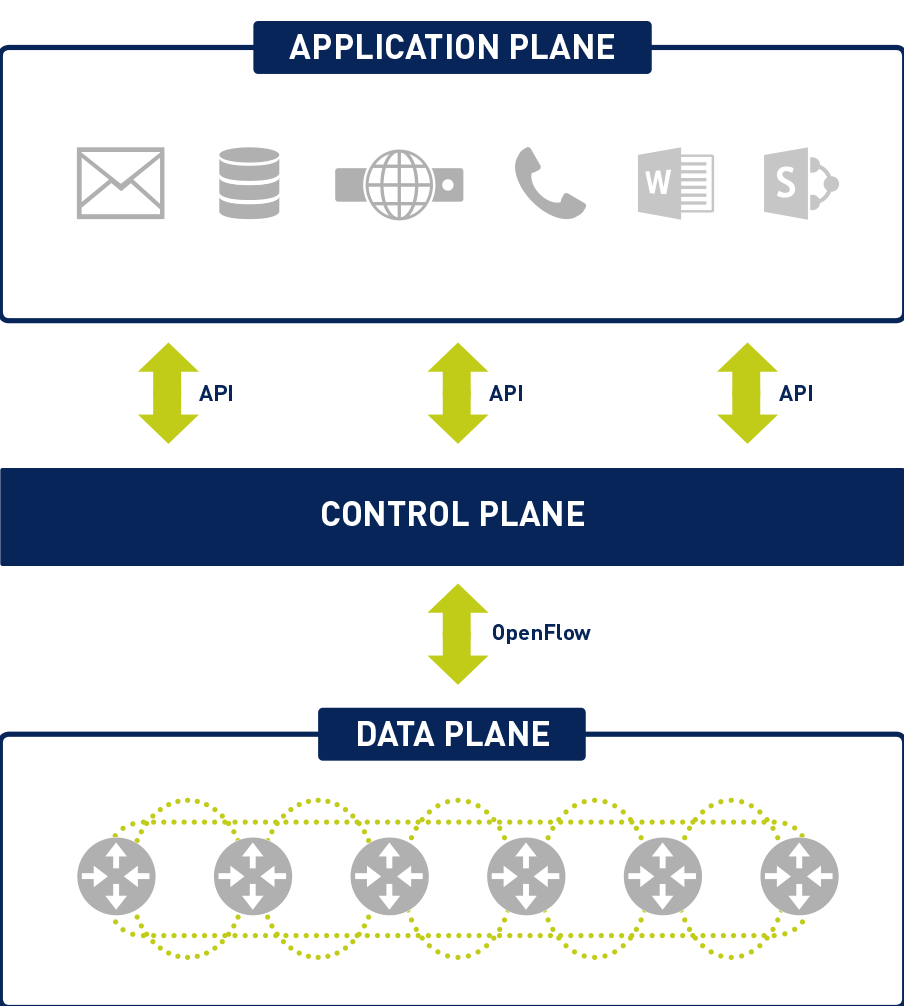
\includegraphics[scale=0.32]{images/sdn.png}
    \caption{\textit{Architettura delle SDN}}
    \label{fig:sdn}
\end{figure}
\FloatBarrier

\subsection*{Control Plane}
\addcontentsline{toc}{subsection}{Control Plane}

Il Control Plane è il piano di controllo adibito a numerosi ruoli.
Nelle SDN che utilizzano OpenFlow \cite{noauthor_openflow}, il Control Plane si occupa della scelta del percorso del pacchetto in rete, della popolazione della Routing Table e della Forwarding Table.
Le nuove reti SDN, invece, puntano alla riprogrammabilità a livello di Data Plane, delegando a questo livello le decisioni sull'instradamento dei pacchetti. P4, ad esempio, riesce a rendere programmabili i dispositivi come gli switch iniettando direttamente le regole per il forwarding e definendo tramite il ``codice P4", che verrà compilato in un eseguibile, le azioni che il dispositivo deve svolgere.\\

\subsection*{Data Plane}
\addcontentsline{toc}{subsection}{Data Plane}
Il Data Plane è la parte effettiva che si occupa del forwarding dei pacchetti. È il livello che si occupa del controllo del flusso reale dei dati che passano in rete.
Generalmente, dopo aver ricevuto direttiva di inoltro da parte del piano di controllo, si applica il forwarding ai pacchetti. A questo livello è fondamentale per la velocità della rete avere degli algoritmi efficaci tali che usino meno risorse possibili. È in questo piano che poniamo DPDK e P4.

\subsection*{Tecnologie Utilizzate e Casi D'Uso}
\addcontentsline{toc}{subsection}{Tecnologie Utilizzate e Casi D'Uso}
Di seguito sono elencate alcune delle tecnologie a livello applicativo nelle quali è possibile introdurre le SDN, in particolare P4 e DPDK. 

\begin{itemize}
    \item \textbf{Indipendenza dai Protocolli}. Le SDN forniscono una programmabilità versatile che permette di specificare il parsing degli header dei pacchetti di dati (anche a runtime), rendendo i programmi, come quelli su switch P4, adattabili al tipo di protocollo adottato.
    \item \textbf{Monitoraggio di Rete}. Fornendo un Data Plane programmabile, con P4 è possibile monitorare e analizzare il traffico di rete introducendo specifiche regole e azioni da applicare con l'arrivo di determinati header o pacchetti di dati. Un esempio reale è l'introduzione di una DoS protection tramite le SDN \cite{navid_detection_2017}.
    \item \textbf{Distribuzione della Rete}. Con le SDN in generale, ma nello specifico con P4, è possibile costruire una rete virtuale composta da molti nodi, centralizzata e programmabile ``on the fly" che permette di applicare modifiche molto velocemente. Uno caso molto diffuso è quello delle Virtual Private Cloud (VPC) offerte da Amazon Web Services (AWS), ovvero reti virtuali interne che servono per isolare spazi di lavoro \cite{noauthor_aws_sdn}.
    \item \textbf{Controllo della Rete}. Tramite le SDN è possibile applicare ai dati in arrivo le politiche di Load Balancing, Congestion Control e Logging così da gestire la rete mantenendone il massimo controllo. Queste soluzioni possono essere adottate a livello Enterprise per avere un alto livello di ``Governance" sulle proprie reti interne. Un chiaro esempio di Load Balancing basato su SDN è il SLB (Software Load Balancer) di Microsoft Azure \cite{noauthor_azure_sdn}.
    \item \textbf{Velocità di trasmissione}. Con DPDK è possibile trasmettere dati ad una velocità elevata anche utilizzando hardware di basso costo, rendendo così le SDN adattabili a tecnologie di uso quotidiano. Un caso di utilizzo di DPDK a livello Server è nell'introduzione di questa tecnologia nei Data Center di Lenovo \cite{noauthor_lenovo_sdn}.
\end{itemize}





